\documentclass[12pt,a4paper]{article}

\usepackage[utf8]{inputenc}
\usepackage[T1]{fontenc}
\usepackage{lmodern}
\usepackage{amsmath}
\usepackage{graphicx}
\usepackage{caption}
\usepackage{hyperref}
\usepackage[margin=2.0cm]{geometry}
\usepackage{titlesec}
\usepackage{enumitem}

\titlespacing*{\section}{0pt}{8pt plus 2pt}{4pt}
\captionsetup{font=small, labelfont=bf, skip=3pt}
\setlength{\textfloatsep}{8pt plus 2pt}
\setlength{\parskip}{3pt}
\setlength{\parindent}{0pt}
\setlength{\emergencystretch}{3em}
\setlist{nosep, leftmargin=1.4em}
\sloppy

\begin{document}
\begin{center}
    {\Large\textbf{Sociodynamics of Emutopia and Kiwiland relations}}\\[2pt]
    Collective Intelligence -- Assignment 1 \quad$\cdot$\quad Matyas Patacsi, YA1O1L \quad$\cdot$\quad \today

\end{center}
\vspace{-0.6cm}

%% ===================================================================== PAGE 1
\section{Model summary}
\textbf{Topic:} In this work, a fictional conflict between Emutopia and Kiwiland is examined. Emutopia is attempting to send ``airborne humanitarian food deliveries'' to Kiwiland, which the latter does not want to receive as it prefers different cuisines.

\textit{Note: from this point on, the report and work use military terminology, as the situation is surprisingly close to a scenario of that type.}

The focus of this simulation is decoy drones. The attackers mix decoys in with regular armed drones to waste the defender's interceptors. The dynamics of this phenomenon are of interest.

\textbf{Research Question:} How do the decoy share of the attack budget and the defender's ability to recognise decoys decide whether an air defence holds?

\textbf{Hypothesis:} Above some decoy share, the decoys empty the magazines and the losses jump abruptly instead of rising gradually; better decoy recognition moves this tipping point to higher decoy shares.

\textbf{World:} $128\times128$; bases sit in a central homeland; drones launch from a circle around it in waves.

\textbf{Agents and globals:}
\begin{itemize}
    \item \emph{Bases} (4; \texttt{health}, \texttt{ammo} (max 10), \texttt{reload-timer}, \texttt{launch-cooldown}): reload slowly and launch interceptors at drones in radar range.
    \item \emph{Drones} (\texttt{decoy?}, \texttt{target}, \texttt{speed}, \texttt{launched}): fly straight at an assigned base; a lethal hit deals 34 damage (3 destroy a base), a decoy 0.
    \item \emph{Interceptors} (\texttt{target}, \texttt{fuel}): chase one drone, roll for a kill and are used up.
    \item \emph{Globals:} \texttt{raining?}, wave counter, outcome counters.
\end{itemize}

\textbf{Each tick:} launch a wave if due $\rightarrow$ update weather $\rightarrow$ bases reload and launch $\rightarrow$ drones and interceptors move $\rightarrow$ hits are resolved.

\textbf{Design concepts:}
\begin{itemize}
    \item \emph{Sensing:} with probability equal to the decoy recognition, a base targets the nearest \emph{lethal} drone, otherwise the nearest drone of any kind.
    \item \emph{Weather (dynamic environment):} random rain showers lower the kill chance by \texttt{rain-penalty}.
    \item \emph{Saturation (non-trivial rule):} a base can only fire while it has ammo, and its magazine of 10 refills one interceptor every 4 ticks, so a large enough swarm empties it and the remaining drones get through.
\end{itemize}

\textbf{Key parameters:}
\begin{itemize}
    \item \texttt{decoy-ratio} (\textit{swept}): share of the wave budget spent on decoys.
    \item \texttt{sensor-discrimination} (\textit{swept}): \textbf{decoy recognition}, the chance a base recognises lethal drones.
    \item \texttt{wave-budget} / \texttt{decoy-cost} (3750 / 15): budget per wave / price of a decoy (a lethal drone costs 100).
    \item \texttt{intercept-accuracy} (85\%): kill chance per interceptor.
    \item \texttt{base-reload-time} / \texttt{detection-radius} (4 / 26): reload ticks / radar range.
    \item \texttt{rain-chance} / \texttt{rain-penalty} (1\% / 50\%): rain start chance / kill chance lost in rain.
\end{itemize}

\textbf{Interface:} \texttt{setup} / \texttt{go-once} / \texttt{go}; 15 sliders; 6 monitors (weather, ticks, bases left, hits, interceptions); plots of base health and interception outcomes over time; a histogram of drone distances to their target.

\newpage
%% ===================================================================== PAGE 2
\section{Experiments and results}

\textbf{Two-factor design setup:} decoy share $\times$ decoy recognition (561 settings, 100 runs each), other parameters at their defaults. Outcomes: bases destroyed (0--4) and lethal hits. Mean and 95\% CI were computed for all 561 settings; the CIs are at most $\pm0.36$ bases.

\textbf{Parameter ranges:} decoy share 0--100\% (step 2\%) covers every split of the budget, finely enough to resolve the jump at 15--30\%; decoy recognition 0--100\% (step 10\%) spans a blind to a perfect defence, along which the response changes smoothly.

\begin{figure}[h]
    \centering
    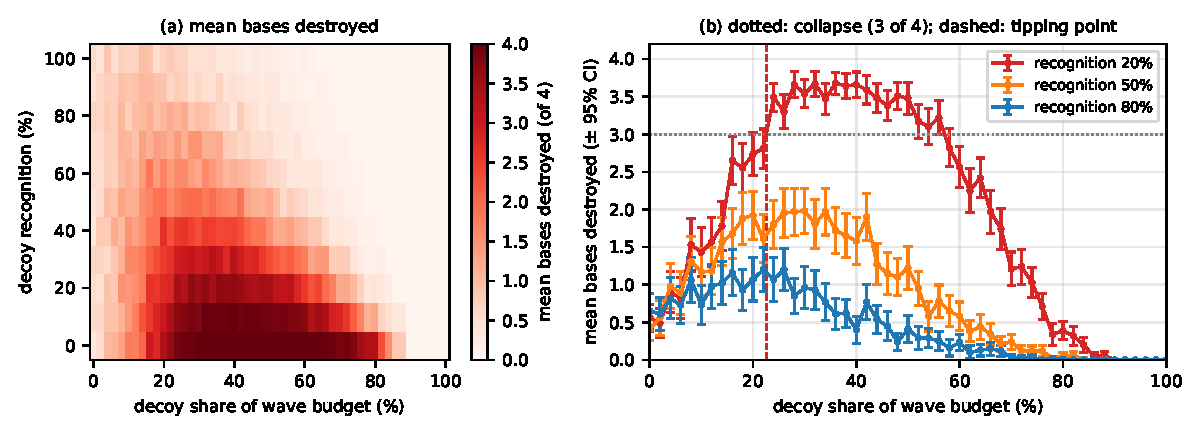
\includegraphics[width=0.85\linewidth]{fig_sweep.pdf}
    \caption{(a) Mean bases destroyed. (b) Means $\pm$ 95\% CI at three levels of decoy recognition; dotted: collapse level (3 of 4 bases), dashed: estimated tipping point.}
    \label{fig:sweep}
\end{figure}

\begin{figure}[h]
    \centering
    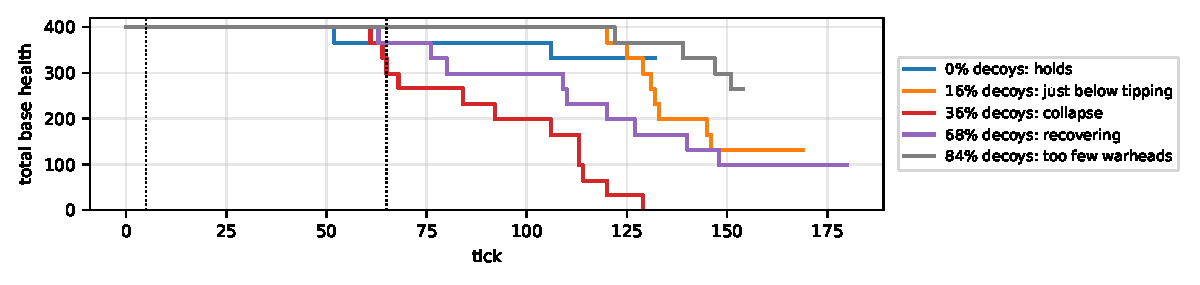
\includegraphics[width=0.84\linewidth]{fig_timeseries.pdf}
    \caption{Total base health at 20\% decoy recognition, median run of 20 per decoy share; dotted lines: wave launches.}
    \label{fig:ts}
\end{figure}

\textbf{Regime change:} We call it collapse when on average at least 3 of the 4 bases are destroyed. At 20\% decoy recognition the tipping point is at \textbf{22.6\%} decoys: losses jump from $0.56\pm0.18$ bases without decoys to $3.54\pm0.19$ at 30\% (Fig.~\ref{fig:sweep}b). Better decoy recognition moves the tipping point up (18.8\% at 0\% recognition, 26.5\% at 30\%), and from 40\% recognition the defence never collapses. After the peak at 36\% the losses fall again and stay below 0.5 bases from 78\% decoys, because too few warheads are left (Fig.~\ref{fig:ts}).

\textbf{Takeaway:} \emph{An air defence that easily handles warheads alone does not degrade gradually but collapses abruptly once about a fifth of the attack budget (roughly two decoys per warhead) is spent on cheap decoys, because the decoys empty its magazines and the remaining warheads get through unopposed; recognising decoys more than about a third of the time prevents this collapse entirely, and only an almost pure decoy swarm is harmless again, as it carries too few warheads.}

\textbf{Limitations:}
\begin{itemize}
    \item \emph{Simple attackers:} drones fly straight without evasion, decoys do no damage, and the attacker never adapts its decoy share.
    \item \emph{Simple defence:} each base fires on its own (no central fire control or shared magazines), and recognising a decoy is one random roll per launch, independent of range or time.
    \item \emph{Narrow scope:} only two factors were swept with everything else at one setting.
    \item \emph{Flat world:} 2D without terrain or altitude; the weather is only rain or no rain.
\end{itemize}

\end{document}
